\documentclass[12pt,letterpaper]{article}
\usepackage[utf8]{inputenc}
\usepackage[spanish]{babel}
\usepackage{graphicx}
\usepackage[left=2cm,right=2cm,top=2cm,bottom=2cm]{geometry}
\usepackage{graphicx} % figuras
% \usepackage{subfigure} % subfiguras
\usepackage{float} % para usar [H]
\usepackage{amsmath}
\usepackage{minted}
%\usepackage{txfonts}
\usepackage{stackrel} 
\usepackage{multirow}
\usepackage{enumerate} % enumerados
\renewcommand{\labelitemi}{$-$}
\renewcommand{\labelitemii}{$\cdot$}
% \author{}
% \title{Caratula}
\begin{document}

% Fancy Header and Footer
% \usepackage{fancyhdr}
% \pagestyle{fancy}
% \cfoot{}
% \rfoot{\thepage}
%

% \usepackage[hidelinks]{hyperref} % CREA HYPERVINCULOS EN INDICE

% \author{}
\title{Caratula}

\begin{titlepage}
\begin{center}
\large{UNIVERSIDAD PRIVADA DE TACNA}\\
\vspace*{-0.025in}
\begin{figure}[htb]
\begin{center}

\includegraphics[width=8cm]{./imagenes/logo}
\end{center}
\end{figure}
\vspace*{0.15in}
INGENIERIA DE SISTEMAS  \\

\vspace*{0.5in}
\begin{large}
TITULO:\\
\end{large}

\vspace*{0.1in}
\begin{Large}
\textbf{INFORME DE LABORATORIO N 05} \\
\end{Large}

\vspace*{0.3in}
\begin{Large}
\textbf{CURSO:} \\
\end{Large}

\vspace*{0.1in}
\begin{large}
INTELIGENCIA DE NEGOCIOS\\
\end{large}

\vspace*{0.3in}
\begin{Large}
\textbf{DOCENTE(ING):} \\
\end{Large}

\vspace*{0.1in}
\begin{large}
 Patrick Cuadros Quiroga\\
\end{large}

\vspace*{0.2in}
\vspace*{0.1in}
\begin{large}
Integrantes: \\
\begin{flushleft}
Layme Valeriano Diego 		\hfill	(2017057865) \\
\end{flushleft}
\end{large}
\end{center}

\end{titlepage}


\tableofcontents % INDICE
\thispagestyle{empty} % INDICE SIN NUMERO
\newpage
\setcounter{page}{1} % REINICIAR CONTADOR DE PAGINAS DESPUES DEL INDICE DE CUESTIONARIO

\section{TAREA 1: IMPORTACION DE DATOS USANDO EL WIZARD – SQL MANAGMENT} 

\begin{enumerate}
    \item Crear una base de datos – BDTEST
        \begin{center}
             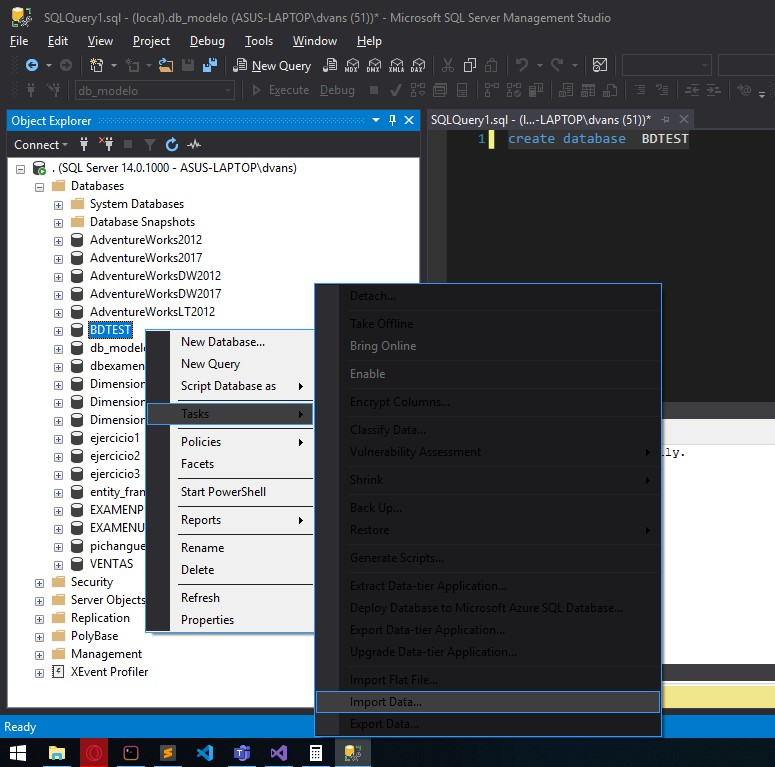
\includegraphics[width=10cm]{imagenes/importa_data_1.jpg}
        \end{center}
        
     \item Elegimos la base de datos origen
        \begin{center}
             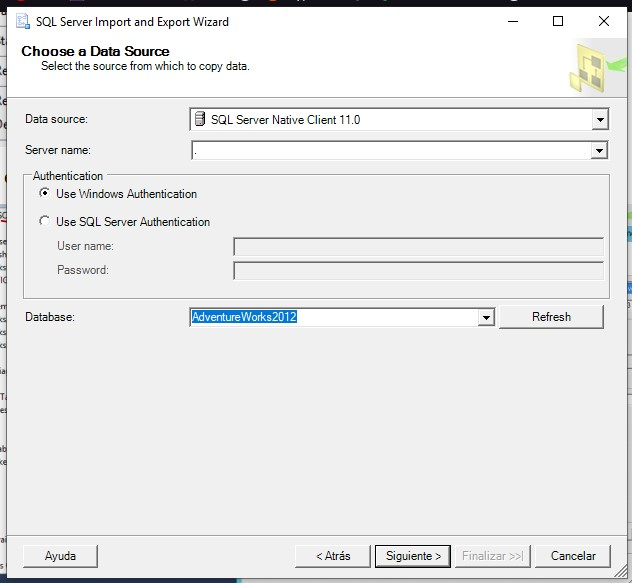
\includegraphics[width=10cm]{imagenes/importa_data_2.jpg}
        \end{center}
        
        \newpage
        
     \item Elegimos la base de datos destino
        \begin{center}
             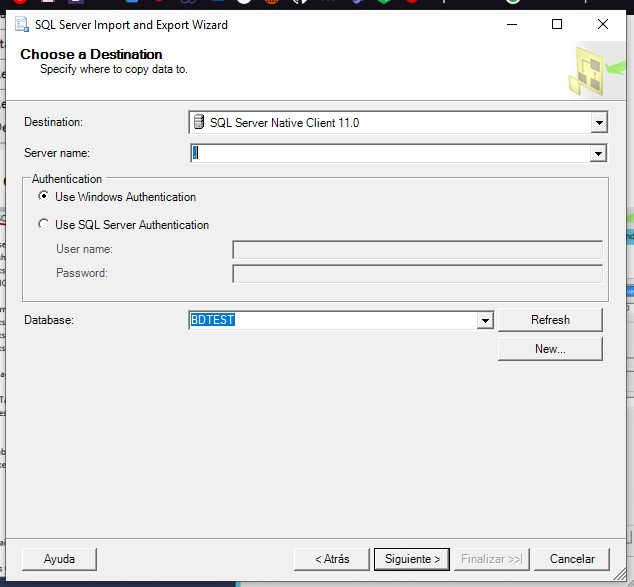
\includegraphics[width=10cm]{imagenes/importa_data_3.jpg}
        \end{center}
        
     \item Selecionamos la primera opcion
        \begin{center}
             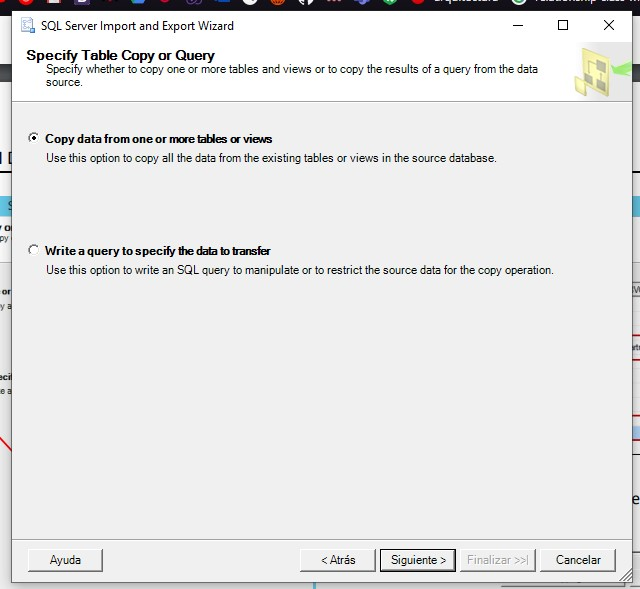
\includegraphics[width=10cm]{imagenes/importa_data_4.jpg}
        \end{center}
        \newpage
        
     \item Selecionamos las tablas Human.Deparment y Person.Address
        \begin{center}
             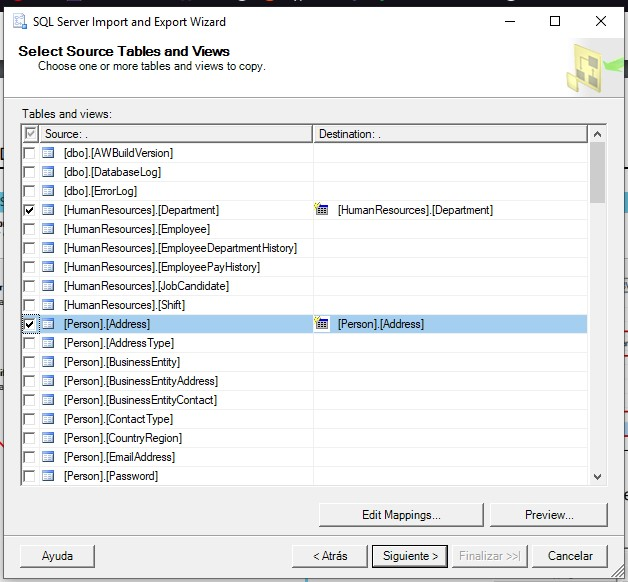
\includegraphics[width=10cm]{imagenes/importa_data_5.jpg}
        \end{center}
        
     \item Activamos para que guarde el paquete
        \begin{center}
             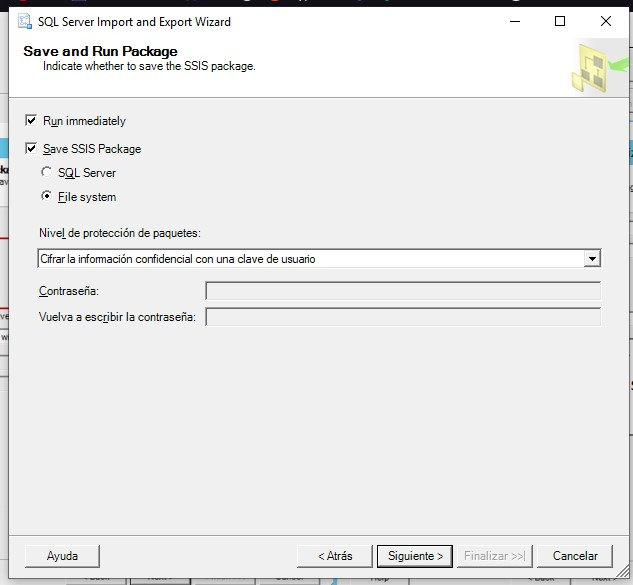
\includegraphics[width=10cm]{imagenes/importa_data_6.jpg}
        \end{center}
        \newpage
        
     \item Asignamos nombre y ruta del archivo
        \begin{center}
             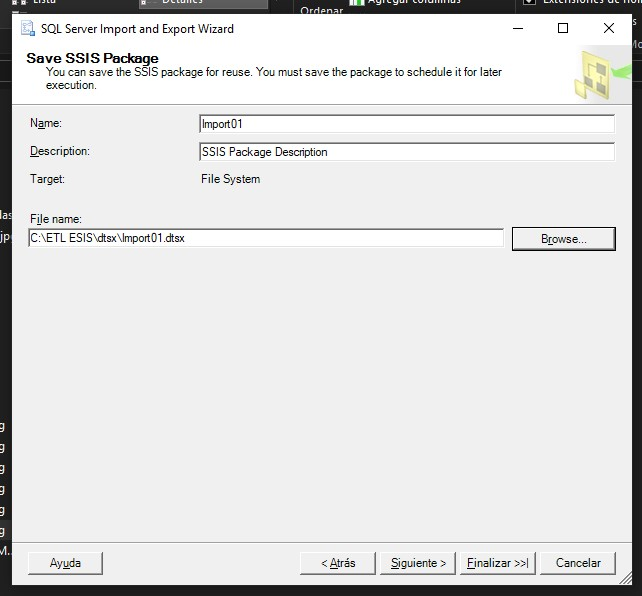
\includegraphics[width=10cm]{imagenes/importa_data_7.jpg}
        \end{center}
        
     \item Presionamos en finalizar
        \begin{center}
             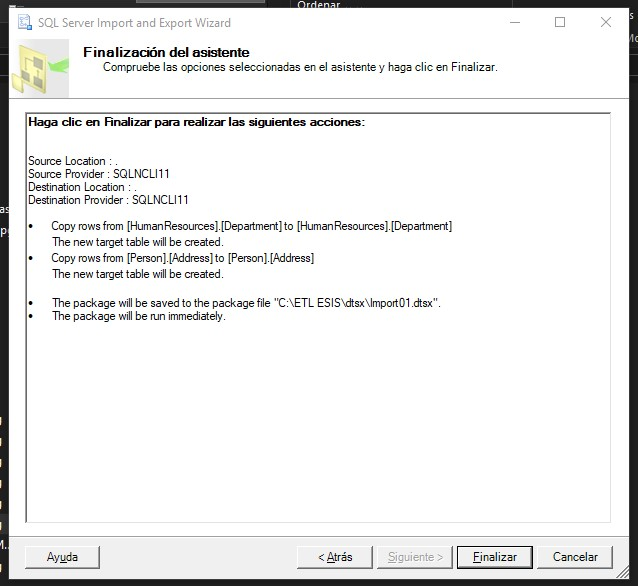
\includegraphics[width=10cm]{imagenes/importa_data_8.jpg}
        \end{center}
        \newpage
                
     \item Una vez terminado el procedimiento , presionamos en el boton Cerrar
        \begin{center}
             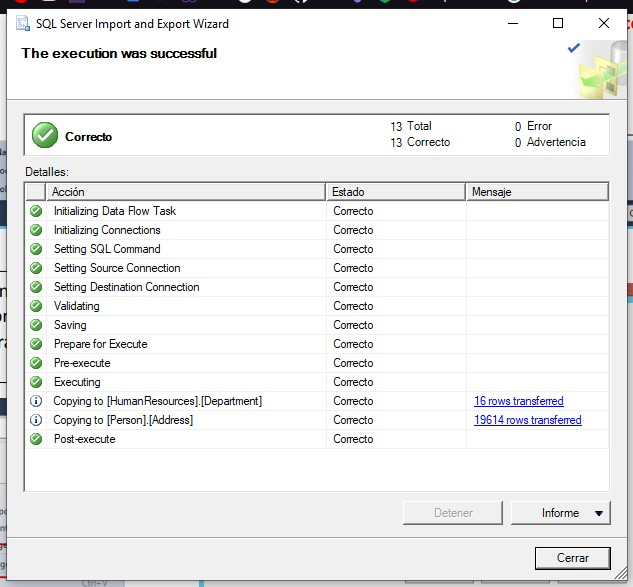
\includegraphics[width=10cm]{imagenes/importa_data_9.jpg}
        \end{center}

\end{enumerate}
\section{TAREA 2: CREAMOS NUESTRO PRIMER PAQUETE DTSX}

\begin{enumerate}
    \item Crear un proecto de Business Intelligense : Integration Services
     \begin{center}
            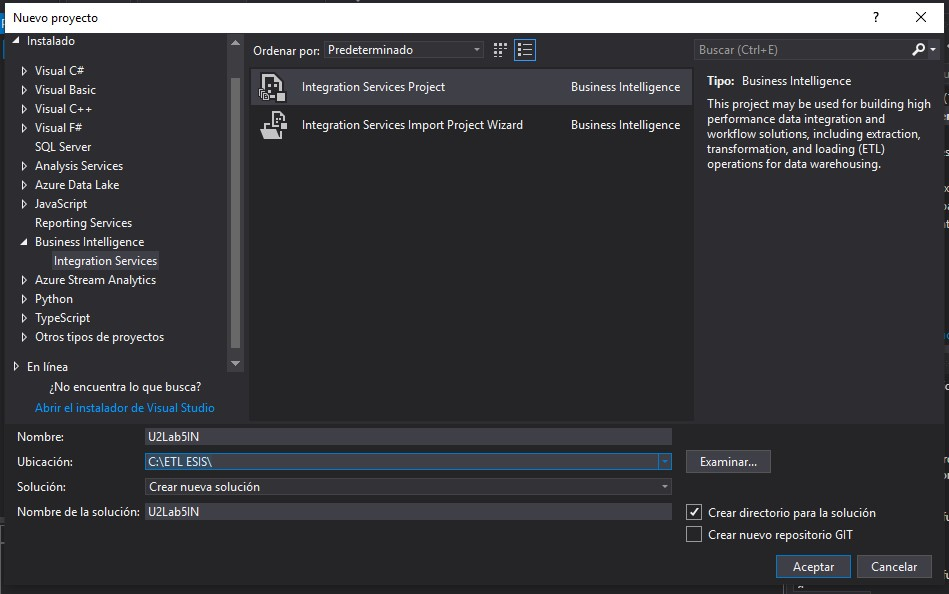
\includegraphics[width=10cm]{imagenes/bi_1.jpg}
        \end{center}
        
    \item Agregamos el paquete Import01.dtsx generado anteriormente
     \begin{center}
            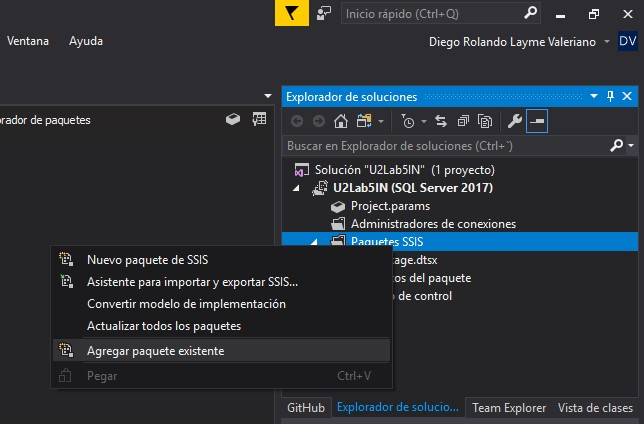
\includegraphics[width=10cm]{imagenes/bi_2.jpg}
        \end{center}
        
        
                
    \item Configuramos una nueva conexion 
     \begin{center}
            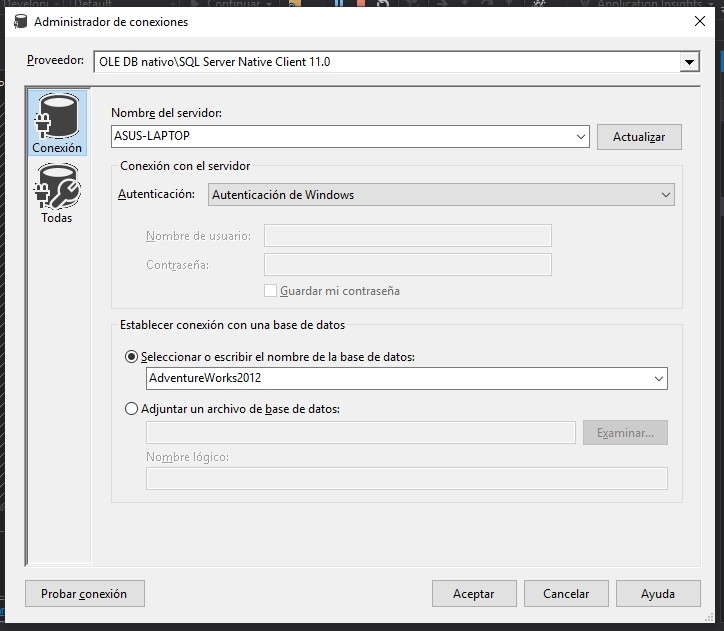
\includegraphics[width=10cm]{imagenes/registros_2_conexion.jpg}
        \end{center}
        
   \item Agregamos una Tarea de flujo de datos y  una tarea de Ejecutar SQL
     \begin{center}
            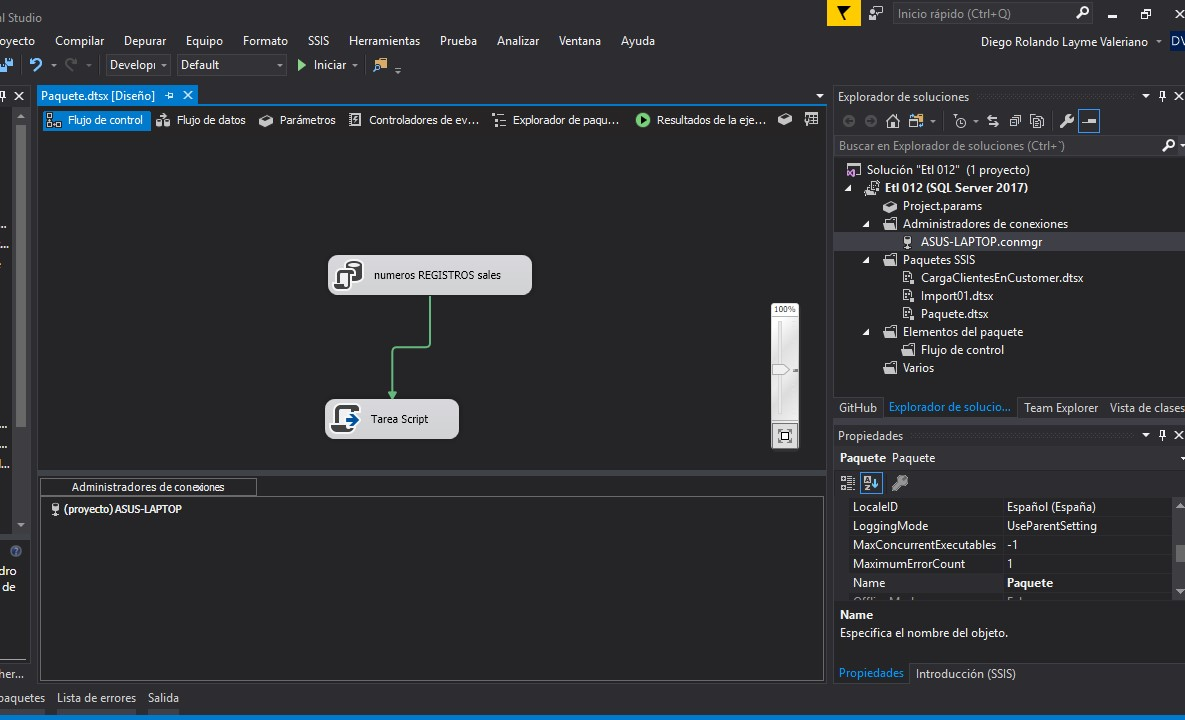
\includegraphics[width=10cm]{imagenes/registros_componentes.jpg}
        \end{center}
        
        
                
    \item Abrimos la Tarea de Ejecutar SQL y configuramos la consulta para obtener la cantidad de registros en SQL Statement
     \begin{center}
            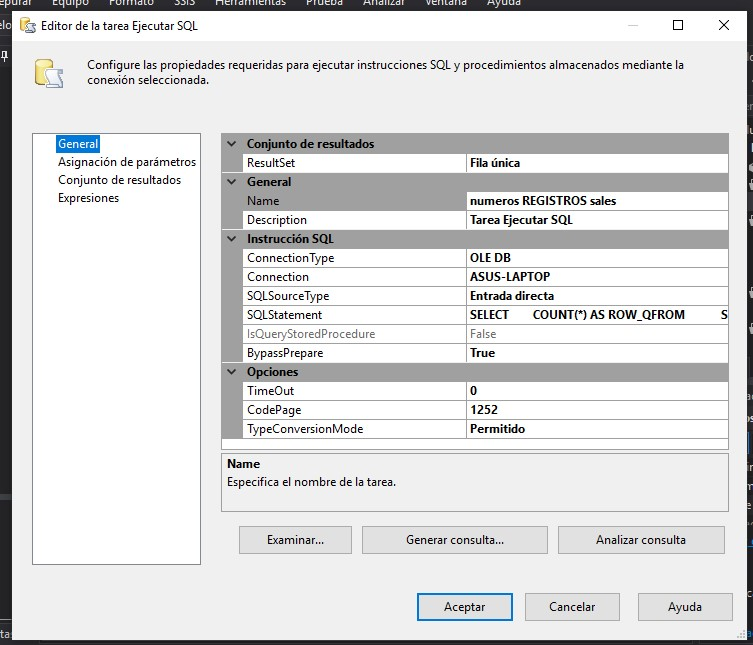
\includegraphics[width=10cm]{imagenes/registros_flujo_configuracion.jpg}
        \end{center}
        
        
                
    \item Asignar la variable en “Numero de Registros Sales”
     \begin{center}
            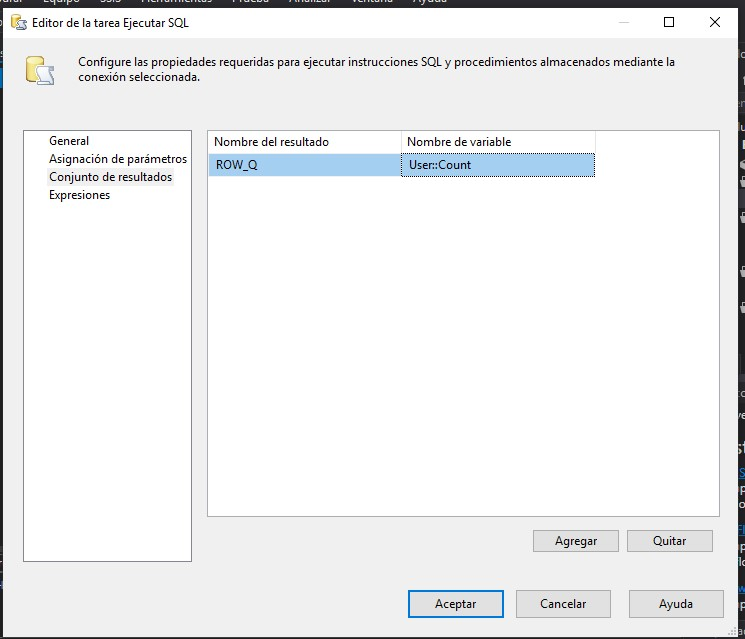
\includegraphics[width=10cm]{imagenes/registros_result_set.jpg}
        \end{center}
        
    \item Editamos el componente Tarea Ejecutar SQL
     \begin{center}
            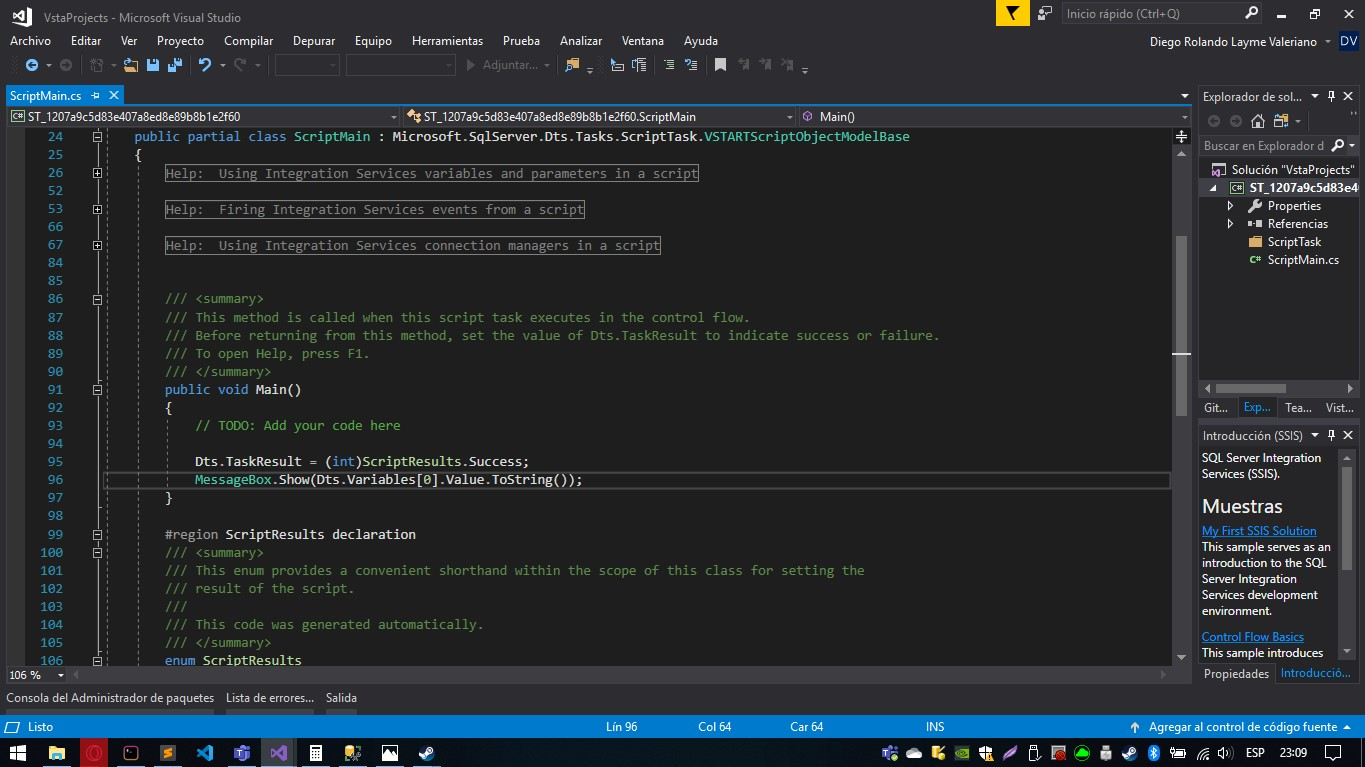
\includegraphics[width=10cm]{imagenes/registros_proyecto_print.jpg}
        \end{center}
        
    \item Finalmente Ejecutamos
     \begin{center}
            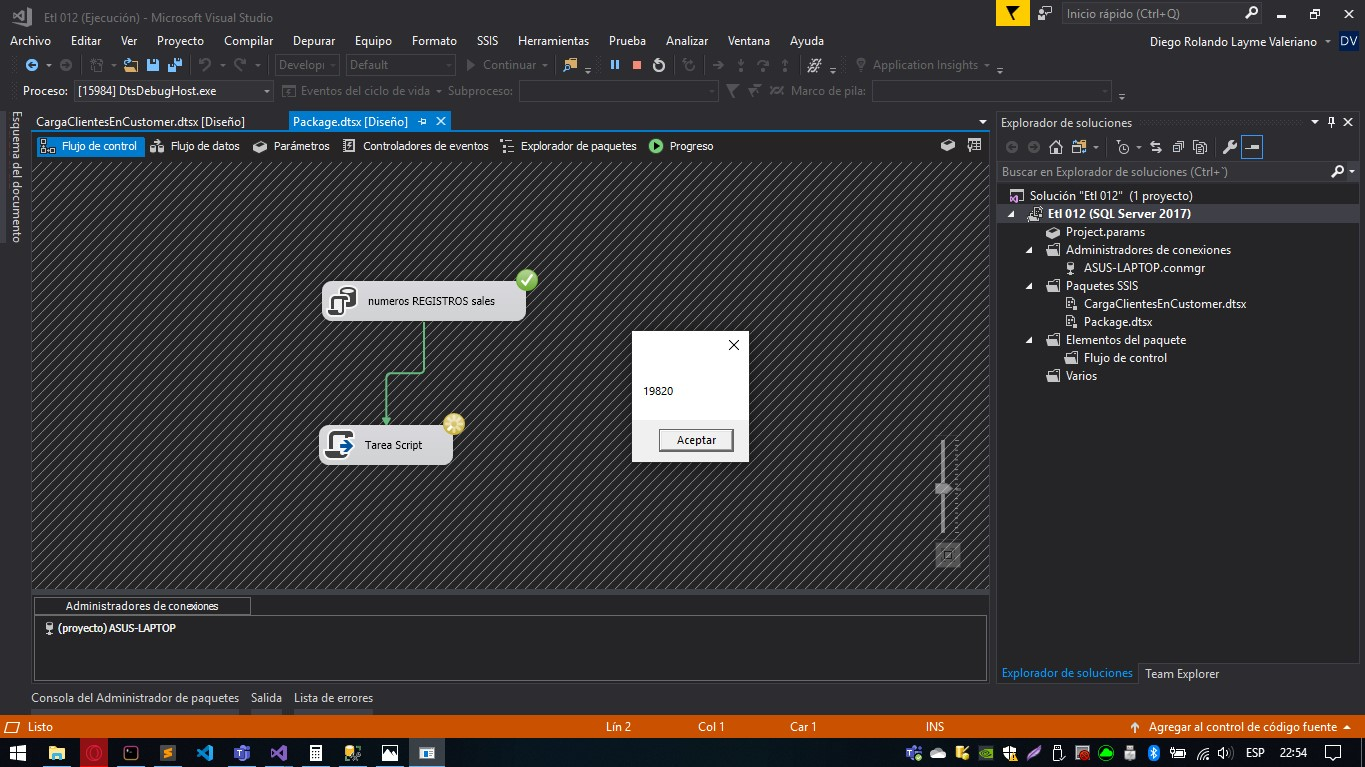
\includegraphics[width=10cm]{imagenes/registros_final.jpg}
        \end{center}
\end{enumerate}




\end{document}